\documentclass{mprop}
\usepackage{graphicx}
\usepackage{amsthm}
\theoremstyle{definition}
\usepackage{mathtools}
\usepackage[numbers]{natbib}
\usepackage{thmtools}
\usepackage[usenames, dvipsnames]{color}
\usepackage{algorithm}
\usepackage{algpseudocode}
\usepackage{hyperref}
\usepackage{caption}
\usepackage{subcaption}
\usepackage{amsfonts}
\usepackage{enumitem}
\usepackage{multirow}

\newtheorem{example}{Example}
\newtheorem{theorem}{Theorem}

\declaretheoremstyle[headfont=\bfseries]{solution}
\declaretheoremstyle[headfont=\normalfont]{normalhead}
\declaretheorem[style=normalhead, numbered=no]{question}
\declaretheorem[style=normalhead, numbered=no]{instance}
\declaretheorem[style=solution, numbered=no]{solution}

\newcommand{\specialcell}[2][c]{%
  \begin{tabular}[#1]{@{}c@{}}#2\end{tabular}}

\def\Item$#1${\item[] $\displaystyle#1$
   \hfill\refstepcounter{equation}(\theequation)}

% alternative font if you prefer
\usepackage{times}

% for alternative page numbering use the following package
% and see documentation for commands
%\usepackage{fancyheadings}


% other potentially useful packages
%\uspackage{amssymb,amsmath}
%\usepackage{url}
%\usepackage{fancyvrb}
%\usepackage[final]{pdfpages}

\begin{document}
\title{The Traveller's Problem}
\author{Iva Stefanova Babukova}
\date{18 December 2016}
\maketitle
\tableofcontents
\educationalconsent
\newpage

%%%%%%%%%%%%%%%%%%%%%%%%%%%%%%%%%%%%%%%%%%%%%%%%%%%%%%%%%%%%%%%%%%%
\section{Introduction}
\label{intro}
The Traveller’s Problem (TP) is a combinatorial optimisation problem whose extensions and variations are often encountered by travellers around the world.
Given a set of airports, a set of flights, a set of destinations that is a subset of the airports, and a special airport $A_{0}$, a solution is a travel schedule that starts and finishes at $A_{0}$, visits all destinations and is in accordance with additional constraints specified by the traveller. For instance, the traveller may wish to spend a certain amount of days in each destination, to take a minimum number of connection flights, or to give minimum amount of money for flights. This work gives a formal description of TP and some of its main extensions, proves a result concerning its complexity, investigates existing methods to solve similar problems and presents a plan of action for modelling TP, generating TP datasets from the Skyscanner flights data and carrying out empirical evaluation.

This work is organised as follows. Section \ref{sec:tpformulation} gives a formal definition of TP and Section \ref{sec:tpexample} presents some example TP instances. Section \ref{npcompleteproblems} lists the formulation of all problems studied in this work. Section \ref{sec:tpcomplexity} justifies the complexity of TP. Section \ref{sec:existingwork} presents the background survey, where we discuss common techniques to solve problems similar to TP with respect to their complexity and formulation. Section \ref{sec:requirements} presents the prioritised project requirements. Our proposed approach is described in Section \ref{sec:proposedapproach}. It includes two distinct models for TP, evaluation plan and a discussion about how datasets for experiments will be created. Finally, Section \ref{sec:workplan} presents a detailed plan of work and time estimation of each task of high priority.

%%%%%%%%%%%%%%%%%%%%%%%%%%%%%%%%%%%%%%%%%%%%%%%%%%%%%%%%%%%%%%%%%%%
\section{Problem Formulation}
\label{sec:tpformulation}

Each instance of TP consists of:

\begin{enumerate}
\item A set of airports $A = \{ A_{0},...,A_{n} \}$ for $n > 0$. Each airport $A_{i}$ $\in$ $A$ represents a location the traveller can begin their commute in, visit as a desired destination, or connect in on the way to their destination.

\item The trip starts and ends at the same airport $A_{0}$, which is referred to as the \textit{home point}.

\item The total travel time $T$, within which the traveller must have visited all destinations and returned to the home point. The first day is day 0.
 
\item A set of flights $F = \{ f_{0},...,f_{m} \}$. Each flight $f_{j}$ has:
\begin{itemize}
\item departure airport $A^{d}_{j}$,
\item arrival airport $A^{a}_{j}$,
\item date $t_{j}$,
\item duration $\Delta_{j}$,
\item cost $c_{j}$,
\end{itemize} 
for some non-negative integer $j$ less than or equal to $n$.
The date $t_{j}$ is a positive rational number less than or equal to $T$ that shows at which day $f_{j}$ leaves its departure airport. The duration $\Delta{j}$ is a positive fraction that shows the amount of time that takes for flight $f_{j}$ to go from $A^{d}_{j}$ to $A^{a}_{j}$. The cost $c_{j}$ is a positive number that denotes the number of units of some currency $\epsilon$ that the traveller pays in order to be able to board flight $f_{j}$.

\item Each airport $A_{i}$ has a \textit{connection time} $C_{A_{i}}$, that is the time that takes to switch from any selected flight $f_{p}$ with $A^{a}_{p} = A_{i}$ to any selected flight $f_{q}$ with $A^{d}_{q} = A_{i}$, where $f_{q}$ is immediately after $f_{p}$ in a solution.

\item A set of \textit{destinations} $D = \{ D_{1},...,D_{l} \}$, $D \subseteq A$, $l \leq n$.
\end{enumerate}

A solution to any instance of TP is a sequence $s$ of $k$ valid flights, $ \langle f_{i_{1}}, f_{i_{2}},...,f_{i_{k}} \rangle \, \subseteq F$, also called a \textit{trip}. We say that $s$ is valid if the flights in $s$ have the following properties:

\begin{enumerate}
\Item $A^{d}_{i_{1}} = A^{a}_{i_{k}} = A_{0}$
\Item $ A^{a}_{i_{j}} = A^{d}_{i_{j+1}},  \quad 0 < j < k  \quad j$
\Item $ t_{i_{j}} + \Delta_{i_{j}} + C_{r} \leq t_{i_{j+1}}, \quad 0 < j \leq k, \quad \textrm{where } r = A^{d}_{i_{j+1}}$
% david mentioned about possibly adding this as a hard constraint?
\Item $t_{i_{k}} + \Delta_{i_{k}} \leq T$
\Item $ \forall D_{p} \in D, \textrm{ } \exists \textrm{ } f_{i_{j}} \in s \textrm{, such that } A^{a}_{i_{j}} = D_{p} $
\end{enumerate}

In this work, we refer to these properties as \textit{trip properties}. Note that a valid sequence of flights may contain one or more flights to and from airports that are not destinations. Such airports are called \textit{connections}.

% these statements are only really meaningful when you relate TP to TSP and also to VRP.
% \textcolor{red}{Also note that the current problem formulation accepts asymmetric flight costs, i.e. one might have two flights $f_{i}$ and $f_{j}$ such that $A^{d}_{i} = A^{a}_{j}$ and $A^{a}_{i} = A^{d}_{j}$. That does not imply that $c_{i} = c_{j}$. Moreover, the problem formulation does not restrict the flight cost to depend on the flight duration. Consequently, this implies that TP is \textit{asymmetric} and in general the flight cost need not satisfy the \textit{triangle inequality}.}

The \textit{optimization} version of TP (TPO) asks for an \textit{optimal} solution $s$ which minimizes the total sum of the prices of the flights in $s$, denoted by $c(s)$.

The \textit{decision} version of TP (TPD) asks whether there exists a valid sequence of flights $s$, such that $c(s)$ is less than or equal to some given integer $B$. The solution of this problem is a `yes' or `no' answer.

There exist a variety of additional constraints and extensions that can be added to TP. Our problem formulation has only presented the hard constraints which every valid solution to a TP instance must satisfy. In real-world problems, travellers may have additional preferences (soft constraints) and requirements (hard constraints) with regards to their travel. These are discussed in the next two sections.

\subsection{Hard Constraints}
\label{subsec:hardconstraints}
This section presents some additional constraints that might be imposed on a TP instance. If any of them is required, then a solution that does not satisfy the requirement is considered as invalid.

\begin{enumerate}
\item Travellers may wish to spend a certain amount of days at a given destination, specified by both upper and lower bounds. The days may additionally be constrained to be consecutive or not.

\item Travellers may require to spend a given date at a given destination, for example due to an event occurring on that date in this destination.

\item Travellers may require not to fly through a given airport more than once.
\end{enumerate}

\subsection{Soft Constraints}
\label{subsec:softconstraints}
It may be desirable to search for a solution that satisfies some of the following requirements:

\begin{enumerate}
\item Travellers may wish to spend a certain amount $\delta_{i}$ of days in each destination $D_{i}$, where $\delta_{i}$ may be specified as a lower or an upper bound.

\item Travellers may wish to avoid taking connection flights. In such requirement, we wish to maximise the number of flights to and from destinations.

\item Travellers may want to spend as little time on flying as possible. In such case, we wish to find a solution that minimises the sum of the durations of all flights.
\end{enumerate}

%% mention the problem with lexicographic optimisation and multi-objective opimisation
Note that we may have an instance for which all soft constraints can not be satisfied simultaneously. In such case, the traveller may be required to rank his requirements in an order of preference. The instance becomes a lexicographic optimisation problem, where we first optimise the highest ranked objective, and subject to this we optimise the second ranked objective and so on.
If all requirements are equally important for the traveller, we have to solve a multiobjective optimisation problem, where the objectives are all constraints required by the traveller. Each of the objectives is given a weight of importance. The problem is then to optimize the objective function, composed by the constraints, each of them multiplied by its weight. %Multiobjective and lexicographic optimisation problems are discussed later in this work.

Note that most of the aforementioned constraints can be viewed as either hard or soft, depending on the user requirements. It is therefore suggested that any attempt at an investigation of TP assumes as an additional non-functional requirement that any proposed model to solve TP is flexible and can be easily extended by adding, removing and modifying the aforementioned constraints.

\section{Worked Examples}
\label{sec:tpexample}
We present an example instance of TP and comment on some of its solutions.

\begin{example}
\label{example1}
A traveller wishes to visit 4 airports from a set of 7 airports available to travel to and from: 

Glasgow (G), Berlin (B), Milan (M), Amsterdam (A), Paris (P), Frankfurt (F), London (L).

Airport G is the home point, F and L are connections, and B, M, A and P are the destinations. The travel time of the traveller is 15 days. All available flights are listed on Table \ref{table:flights} and the example is shown pictorially on Figure \ref{fig:map}. For simplicity, the duration of each flight is assumed to be 1 day. This means that if the traveller gets a flight at date $x$, they will reach the arrival airport at day $x+1$.

\begin{figure}
\centering
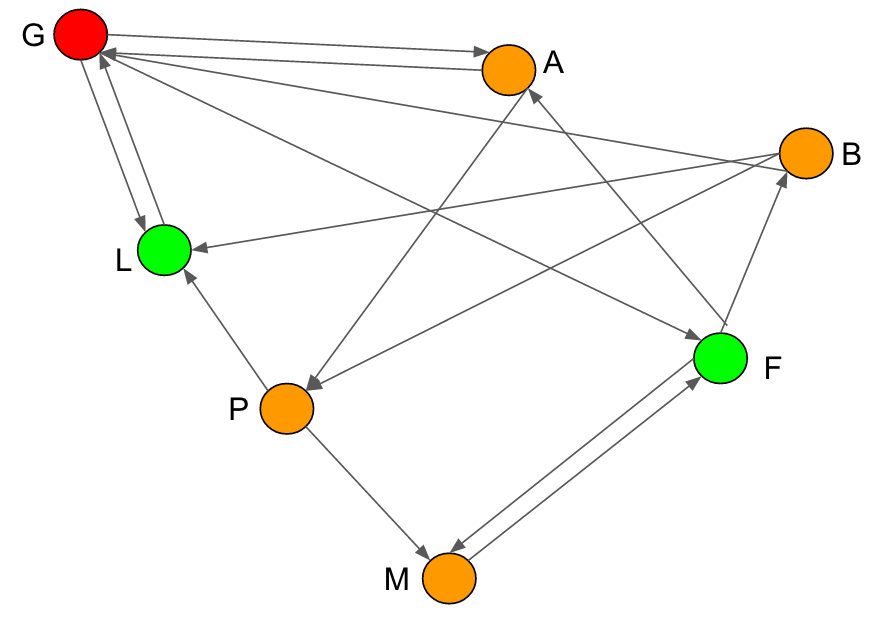
\includegraphics[height=6cm, width=7.5cm]{images/map.png}
\caption{All airports in Example 1. Green vertices are connection airports, orange vertices are destinations and the red vertex is the home point. The links between each two airports are available at certain dates and vary in price, as indicated in Table \ref{table:flights}.}
\label{fig:map}
\end{figure}

\begin{table}
\centering
\renewcommand{\arraystretch}{1.4}% Spread rows out...
\begin{tabular}{|l|l|c|c|c|c|c|}
\hline
& \textbf{Flight No} & \textbf{Departs} & \textbf{Arrives} & \textbf{Date} & \textbf{Price} \\
\hline
1 & GA1 & G & A & \date{1} & 74 \\
\hline
2 & GF1 & G & F & \date{1} & 86 \\
\hline
3 & FB2 & F & B & \date{2} & 156 \\
\hline
4 & GL3 & G & L & \date{3} & 25 \\
\hline
5 & MF3 & M & F & \date{3} & 78 \\
\hline
6 & BP4 & B & P & \date{4} & 67 \\
\hline
7 & AP4 & A & P & \date{4} & 58 \\
\hline
8 & PM6 & P & M & \date{6} & 71 \\
\hline
9 & FM8 & F & M & \date{8} & 234 \\
\hline
10 & MF9 & M & F & \date{9} & 39 \\
\hline
11 & FA10 & F & A & \date{10} & 220 \\
\hline
12 & FB11 & F & B & \date{11} & 122 \\
\hline
13 & FM12 & F & M & \date{12} & 250 \\
\hline
14 & PL12 & P & L & \date{12} & 45 \\
\hline
15 & BG13 & B & G & \date{13} & 335 \\
\hline
16 & BL13 & B & L & \date{13} & 102 \\
\hline
17 & AG13 & A & G & \date{13} & 90 \\
\hline
18 & LG14 & L & G & \date{14} & 24 \\
\hline
\end{tabular}
\caption{List of flights with departure and arrival airports, flight date and price.}
\label{table:flights}
\end{table}
\end{example}

\begin{solution}
A valid solution of the TP instance in the example above is the trip $s$, where the each flight is represented by its flight number, specified in the first column of Table \ref{table:flights}:

$$ s = \langle GA1, AP4, PM6, MF9, FB11, BG13\rangle $$

The total flights cost $c(s)$ is 699.

A valid solution with lower cost is the following trip:

$$ s^{\prime} = \langle GA1, AP4, PM6, MF9, FB11, BL13, LG14\rangle $$

Here $c(s^{\prime})$ is 483 and hence $s$ is not optimal.
\end{solution}

\begin{example}
\label{example2}
Given the same problem instance as in Example \ref{example1}, suppose that the traveller has booked a ticket for a concert in B on day 3. The traveller requires to attend the concert.
\end{example}

\begin{solution}
In such case, neither $s$, nor $s^{\prime}$ from Example \ref{example1} are solutions, because both of them assign the traveller to be at a different location (airport A) at day 3. The following sequence is a solution:

$$ s^{\prime\prime} = \langle GF1, FB2, BP4, PM6, MF9, FA10, AG13\rangle $$

The total cost $c(s^{\prime\prime})$ is equal to 729, which is more expensive than $s$ and $s^{\prime}$.
\end{solution}

\section{Investigated Problems}
\label{npcompleteproblems}

This Section gives a list of known problems, referred to in this work when proving the NP-hardness of TP (Section \ref{npcompleteproof}) and when reviewing the existing work (Section \ref{sec:existingwork}). The problems, marked with an asterisk ($\ast$) next to their title, are known to be NP-complete \citep{thebible}.

\begin{enumerate}

\item \textbf{Vehicle-Routing Problem \textsuperscript{*} (VRP)}
\begin{instance}
A set $A$ of $n$ cities, where $D \in A$ is the \textit{depot} and each city $i$ has demand $c_{i}$, a fleet of $m$ vehicles $V$, where vehicle $k$ has capacity $q_{k}$, a distance $d(i,j)$ between two cities $i$ and $j$ and a positive integer $B$.
\end{instance}

\begin{question}
Is there a set $\mathcal{S}$ consisting of $m$ sequences $s_{1},...,s_{m}$, of the cities in $A$, called \textit{tours}
where for every vehicle $k$ $(1 \leq k \leq m)$:
\begin{itemize}
\item $s_{k} = \langle A_{s_{k,1}},...,A_{s_{k,p_{k}}} \rangle$, \quad where $p_{k}$ is the number of the cities in the tour of $k$,
\item $\sum_{i = 1}^{p} c_{A_{s_{k,i}}} \leq q_{k}$,
\item $A_{s_{k,1}} = D$,
\item $s_{i} \cap s_{j} = \{D\}$, \quad $(1 \leq i < j \leq m),$
\item $s_{1} \cup s_{2} ... \cup s_{m} = A$,
\end{itemize}
and
$$ \sum_{k=1}^{m} C(s_{k}) \leq B \textrm{, where } C(s_{k}) = \bigg( \sum_{i=1}^{p_{k}} d(A_{s_{k,i}}, A_{s_{k,i+1}}) \bigg) + d(A_{s_{k,k_{p}}}, A_{s_{k,1}}) \textrm{ ?}$$
\end{question}


\item \textbf{Travelling Salesman Problem \textsuperscript{*} (TSP) \footnote{Note that TSP is a special case of VRP when only one vehicle is allowed.}}
\begin{instance}
Set $A$ of $n$ cities, distance $d(A_{i}, A_{j})$ between each pair of cities $A_{i}$, $A_{j}$ $\in$ $A$, positive integer $B$.
\end{instance}

\begin{question}
Is there a tour of $A$ having length $B$ or less, i.e., a permutation of cities $\gamma = \langle A_{\pi_{1}},...,A_{\pi_{n}} \rangle $ of $A$ such that the total travel distance $L_{\gamma}$:
$$L_{\gamma} = \bigg( \sum_{i=1}^{n-1} d(A_{\pi_{i}}, A_{\pi_{i+1}}) \bigg) + d(A_{\pi_{n}}, A_{\pi_{1}}) \leq B \quad \textrm{?}$$
\end{question}

\item \textbf{Travelling Salesman Problem Under the Triangle Inequality\textsuperscript{*} (TSP-$\Delta$) \footnote{Note that this problem is a special case of TSP.}}
\begin{instance}
Set $A$ of $n$ cities, distance $d(A_{i}, A_{j})$ between each pair of cities $A_{i}$, $A_{j}$ $\in$ $A$ that satisfies the triangle inequality, positive integer $B$.
\end{instance}

\begin{question}
Is there a tour of $A$ having length $B$ or less, i.e., a permutation of cities $\gamma = \langle A_{\pi_{1}},...,A_{\pi_{n}} \rangle $ of $A$ such that the total travel distance $L_{\gamma}$:
$$L_{\gamma} = \bigg( \sum_{i=1}^{n-1} d(A_{\pi_{i}}, A_{\pi_{i+1}}) \bigg) + d(A_{\pi_{n}}, A_{\pi_{1}}) \leq B \quad \textrm{?}$$
\end{question}

\item \textbf{Time-Constrained TSP\textsuperscript{*} (TCTSP) \footnote{Note that this problem is a generalisation of TSP.}}

\begin{instance}
Set $A$ of $n$ cities, distance $d(A_{i}, A_{j})$ between each pair of cities $A_{i}$, $A_{j}$ $\in$ $A$, positive integer $B$, lower and upper bounds $l_{i}$ and $u_{i}$ respectively for each city $A_{i}$ that specify its time window, where time is a scalar transformation of distance.
\end{instance}

\begin{question}
Is there a permutation of cities $\gamma = \langle A_{\pi_{1}},...,A_{\pi_{n}} \rangle$ of $A$, such that each city $A_{\pi_{i}}$ is visited at time $t_{\pi_{i}}$, where $l_{\pi_{i}} \leq t_{\pi_{i}} \leq u_{\pi_{i}}$, $t_{\pi_{i}} \geq t_{\pi_{i-1}} + d(A_{\pi_{i-1}},A_{\pi_{i}})$ for $(2 \leq i \leq n)$, $t_{\pi_{1}} \geq t_{\pi_{n}} + d(A_{\pi_{n}},A_{\pi_{1}})$,
 and 
$$L_{\gamma} = \bigg( \sum_{i=1}^{n-1} d(A_{\pi_{i}}, A_{\pi_{i+1}}) \bigg) + d(A_{\pi_{n}}, A_{\pi_{1}}) \leq B \quad \textrm{?}$$

\end{question}

\item \textbf{Job-Shop Scheduling Problem\textsuperscript{*} (JSSP)}
\begin{instance}
A set $R$ of resources and a set $N$ of jobs. Each job $J \in N$ consists of a sequence of operations $O_{J}$, a ready time $rt_{J}$ and a deadline $dt_{J}$. Each operation $i$ has processing time $p_{i}$ and required resource $r_{i}$.
\end{instance}

\begin{question}
Is there a sequence $S = \{st_{i} : i \in J, \forall J \in N\}$ of starting times for every operation, such that every job meets its deadline and each resource is used by no more than one job at the same time?
\end{question}

\item \textbf{Time-Constrained Vehicle Routing Problem\textsuperscript{*}
(TCVRP) \footnote{Note that this problem is a generalisation of VRP.}}
\begin{instance}
A set $A$ of $n$ cities, where $D \in A$ is the \textit{depot} and each city $i$ has demand $c_{i}$, a fleet of $m$ vehicles $V$, where vehicle $k$ has capacity $q_{k}$, a distance $d(i,j)$ between two cities $i$ and $j$, lower and upper bounds $l_{i}$ and $u_{i}$ respectively for each city $i$ that specify its time window, where time is a scalar transformation of distance, and a positive integer $B$.
\end{instance}

\begin{question}
Is there a set $\mathcal{S}$ consisting of $m$ sequences $s_{1},...,s_{m}$, of the cities in $A$, called \textit{tours}
where for every vehicle $k$ $(1 \leq k \leq m)$:
\begin{itemize}
\item $s_{k} = \langle A_{s_{k,1}},...,A_{s_{k,p_{k}}} \rangle$, \quad where $p_{k}$ is the number of the cities in the tour of $k$,
\item $\sum_{i = 1}^{p} c_{A_{s_{k,i}}} \leq q_{k}$,
\item $A_{s_{k,1}} = D$,
\item $s_{i} \cap s_{j} = \{D\}$, \quad $(1 \leq i < j \leq m),$
\item $s_{1} \cup s_{2} ... \cup s_{m} = A$,
\item each city $A_{s_{k,i}}$ is visited at time $t_{s_{k,i}}$ with $l_{s_{k,i}} \leq t_{s_{k,i}} \leq u_{s_{k,i}}$,
\item $t_{s_{k,i}} \geq t_{s_{k,i-1}} + d(A_{s_{k,i}},A_{s_{k,i-1}})$, \quad $(2 \leq i \leq n) \footnote{We do not care about the time window on the depot}$,
\end{itemize}
and
$$ \sum_{k=1}^{m} C(s_{k}) \leq B \textrm{, where } C(s_{k}) = \bigg( \sum_{i=1}^{p_{k}} d(A_{s_{k,i}}, A_{s_{k,i+1}}) \bigg) + d(A_{s_{k,k_{p}}}, A_{s_{k,1}}) \textrm{ ?}$$
\end{question}

\item \textbf{The Assignment Problem (AP)}
\begin{instance}
Set $A$ and set $B$ with equal size, cost $c(a,b)$ of matching $a \in A$ to $b \in B$.
\end{instance}

\begin{question}
Find a bijection $f: A \gets B$ such that $\sum_{a\in A} c(a,f(a))$ is minimised.
\end{question}

\end{enumerate}

%%%%%%%%%%%%%%%%%%%%%%%%%%%%%%%%%%%%%%%%%
\section{Complexity of TP}
\label{sec:tpcomplexity}
We state a theorem about the complexity of TP and prove it.
\begin{theorem}
TPD is NP-complete.
\end{theorem}

\begin{proof}
\label{npcompleteproof}
This proof first shows the membership of TPD in the NP class of problems. Second, we prove the NP-hardness of TP by constructing a polynomial-time reduction from a known NP-complete problem $\Pi$ to TPD, where $\Pi$ is chosen to be TSP, defined in Section \ref{npcompleteproblems}. Its NP-hardness follows by a reduction from the Hamiltonian Cycle problem. The proof is presented by \citet{thebible}.

Given an instance of TPD and $s$, which is a sequence of flights from $F$, we can write an algorithm that checks in polynomial time whether $s$ is a solution. To accept or reject validity, the algorithm only needs to traverse $s$ and check that it satisfies all required properties. Therefore, TP is in NP.

Let $\pi$ be an instance of TSP. Let $\pi^{\prime}$ be an instance of TPD with the following properties:
\begin{itemize}
\item The set of airports in $\pi^{\prime}$ is identical to the set of cities in $\pi$ and it is similarly denoted as $A$ (a city in $\pi$ is called an airport in $\pi^{\prime}$). Airport $A_{1}$ is the home point.
\item Each airport in $A$ is also a destination.
\item The connection time $C_{A_{i}}$ for each airport $A_{i}$ is equal to 0.
\item $T$ is equal to $n$.
\item Let $C$ be the Cartesian product of the airports in $A$ with itself, that is $C = A \times A$ = \{($A_{i}, A_{j}$) : $A_{i}$ $\in$ $A$, $A_{j}$ $\in$ $A$, $i \neq j$\}. Then $F$ is a set of flights, such that for every ($A_{i}, A_{j}$) $\in$ $C$, there exists a flight $f_{k}$ in $F$, such that $A^{d}_{k} = A_{i}$ and $A^{a}_{k} = A_{j}$ for every date $0 \leq t < T$.
\item For every $f_{k}$ $\in$ $F$, $c_{k}$ is equal to $d(A^{d}_{k}, A^{a}_{k})$ in $\pi$. Therefore, the flight costs also satisfy the triangle inequality.
\item For every $f_{k}$ $\in$ $F$, $\Delta_{k}$ = 1.
\item $B$ is the upper bound on the allowed total cost.
\end{itemize}

%% TSP solution => also TP solution

Suppose that $\gamma$ = $ \langle A_{i_{1}}, A_{i_{2}},...,A_{i_{n}} \rangle $ is a solution to $\pi$, where $\langle i_{1},...,i_{n} \rangle$ is a permutation of $\langle 1,...,n \rangle $ and the total travel distance $L_{\gamma} \leq B$. Without loss of generality, assume that $i_{1} = 1$. In $\pi^{\prime}$, $\gamma$ is equivalent to the order of visited airports by some sequence of flights $s$ = $ \langle f_{j_{1}}, f_{j_{2}},...f_{j_{n}} \rangle $, such that for each $p$  $(1 \leq p \leq n)$ there exists $q$ $(1 \leq q \leq n)$ such that $A^{d}_{j_{q}} = A_{i_{p}}$ and $A^{a}_{j_{q}} = A_{i_{p+1}}$, where subscripts are taken modulo $n$. Therefore, $s$ satisfies property (1) of a valid solution. For each $q$ $(1 \leq q \leq n)$, $A^{a}_{j_{q}} = A^{d}_{j_{q+1}}$ and $t_{j_{q}} = q - 1$.  We know that such flights exist in $F$ by the construction of the set $F$.

From the construction of $s$, it follows that property (2) also holds. Properties (3) and (4) also hold, since we have chosen flights from $F$ such that for every $f_{j_{q}}$ $\in$ $s$, $t_{j_{q}} = q - 1$ ($(1 \leq q \leq n)$). Property (5) is satisfied, since all airports in $A$ are destinations.

Since the cost of every flight in $F$ is equal to the distance between the two cities in $\pi$ that correspond to its departure and arrival airport, it follows that $c(s) = L_{\gamma} \leq B$.

The sequence $s$ satisfies all requirements for a valid solution to $\pi^{\prime}$. Therefore, a solution of $\pi$ is also a solution to $\pi^{\prime}$.

Conversely, suppose that $s = \langle f_{j_{1}},...,f_{j_{k}} \rangle $ is a solution to $\pi^{\prime}$, where the flights in $s$ visit destinations in the sequence $\gamma^{\prime}$ = $\langle A_{i_{1}}, A_{i_{2}},...,A_{i_{m}} \rangle$. We will prove that $\gamma^{\prime}$ is a solution of $\pi$.

By construction of $\pi^{\prime}$, all airports in $A$ are also destinations. Therefore, $\gamma^{\prime}$ contains all cities in $A$, that is $m \geq n$. Suppose that $m > n$ and an arbitrary airport $A_{p}$ $(1 \leq p < n)$ is included more than once in $\gamma^{\prime}$. Then $s$ must contain more than one flight with arrival airport equal to $A_{p}$. 
The duration of each flight in $\pi^{\prime}$ is one day. Therefore, for every $q$ $(1 \leq q < n - 1)$, $t_{j_{q+1}} = q$. Since the traveller has only $n$ days of total travel time, and $s$ is restricted to contain exactly $n$ flights, that is $k = n$. The only way to visit $n$ distinct destinations, given $n$ flights is that all flights in $s$ have unique arrival airports. Assuming that $A_{p}$ is visited more than once means that there is more than one flight with arrival airport equal to $A_{p}$, which is a contradiction. Therefore, $m = n$ and each airport in $A$ is visited exactly once.

From the properties of $s$ it follows that $A^{d}_{j_{1}} = A^{a}_{j_{n}} = A_{1}$. Therefore, $\gamma^{\prime}$ is a cycle of size $n$. We know that $c(s) \leq B$. We assigned a cost of each flight $f_{k}$ in $F$ to be equal to $d(A^{d}_{k}, A^{a}_{k})$ in $\pi$. Therefore, the total travel distance $L_{\gamma^{\prime}} = c(s)$ which is less than or equal to $B$.

According to the specifications of $\pi$, $\gamma^{\prime}$ is a solution to $\pi$. Therefore, a solution to $\pi^{\prime}$ is also a solution to $\pi$.

The transformation from a TSP instance to an instance of TPD can be done in polynomial time. For each of the $n$($n$-1)/2 distances d($A_{i}$, $A_{j}$) that must be specified in $\pi$, it is sufficient to check that the same cost is assigned to the flights from $A_{i}$ to $A_{j}$ for all dates.

Therefore, TP is in NP and the decision version of TSP can be reduced to TPD in polynomial time, from which it follows that TPD is NP-complete.

\end{proof}

%%%%%%%%%%%%%%%%%%%%%%%%%%%%%%%%%%%%%%%%%%%%%%%%%%%%%%%%%%%%%%%%%%%
\section{Background Survey}
\label{sec:existingwork}
This section presents a detailed review of some existing methods to approach NP-hard problems. In Section \ref{ip} we model TSP as a system of linear integer inequalities and showed a method for computing a lower bound on the cost of the tour that is widely used in the literature. Section \ref{cp} introduces Constraint Programming, where we discuss heuristics and give an example of how heuristics can be specifically designed for a given problem, using JSSP. In Section \ref{sec:tctspalgos} and Section \ref{sec:tcvrpalgos} we discuss some main approaches to solve two NP-hard problems that are somewhat similar to TP, namely TCTSP and TCTSP.
We study 4 different NP-hard problems: TSP, JSSP, TCTSP and TCVRP, all defined in Section \ref{npcompleteproblems}. The purpose of this is to identify successful techniques to model and solve hard problems that could be applied to TP.

\subsection{Branch and Bound Algorithms}
\label{branchandbound}
%In this section we present a branch and bound based solutions for the TCTSP problem.

The term ``branch and bound'' was first coined by \citet{Little63} and it refers to a widely-used method for solving optimisation problems. Given an instance $\pi$ of an optimisation problem, the method repeatedly breaks up the set of candidate solutions into successively smaller subsets, called \textit{subproblems} and calculates a bound on their value. If the bound of a subproblem  is ``worse'' than the best one found so far, the subproblem is discarded. Otherwise, it is added for future investigation. If its bound is the ``best'' found so far, its value is remembered and used for comparison with future subproblems. The process of generating subproblems is called \textit{branching}. We illustrate the branch and bound procedure with the next example.

%The subproblems can be represented as the leaves of a rooted tree $T$, where the root of $T$ is $\pi$, each branch of $T$ represents an assignment of one variable and a node that has a child and is not the root node is called a \textit{branching node}. Branching node represents a partial solution of $\pi$.

\begin{example}
\label{ex:bandb}
Let $\pi$ be the following problem:

$$ \textrm{minimise } x + y \textrm{,}$$

where $x \in \{1, 3, 6\}$ and $y \in \{0, 5\}$.

Figure \ref{fig:bandb} illustrates two possible executions of the branch and bound procedure, depending on the branching rule. Each execution is represented by a tree, where nodes represents subproblems and edges represents variable assignments. The root represents the entire solution set, the green node is an optimum, red nodes denote subproblem sets that were discarded because they have bounds that are ``worse'' compared to the ``best'' bound found so far. Without loss of generality, we assume that the nodes in each tree are visited in a pre-order traversal. For each node $i$ that represents a partial solution, a lower bound $l_{i}$ on its value is calculated, where $l_{i}$ is the sum of the value of all assigned variables. If $i$ represents a single feasible solution, an upper bound $u_{i}$ is calculated, equal to the sum of the assigned value to each variable.

In the left-most tree, the branching rule explores the feasible solutions, assigning values for $x$ and $y$ in a non-increasing order. One can see that it needs to check all possible assignments of $x$ and $y$ in order to find an optimum. This is due to the poor choice of branching rule, which leads to a series of ineffective bounds which can not discard subproblems.

The right-most tree has branching rule that explores the feasible solutions, assigning values for $x$ and $y$ in a non-decreasing order. This is more efficient branching rule for $\pi$, since the size of the tree is smaller. This is because the first encountered feasible solution is an optimal assignment for $x$ and $y$, which sets $1$ as an upper bound on the value of the feasible solutions, which discards partial solutions.

\begin{figure}
\centering
\begin{minipage}{.5\textwidth}
\centering
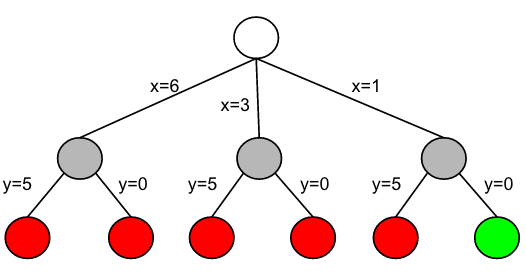
\includegraphics[width=4.5cm, height=2.4cm]{images/fullsearch.png}
\end{minipage}%
% \begin{minipage}{.3\textwidth}
% \centering
% 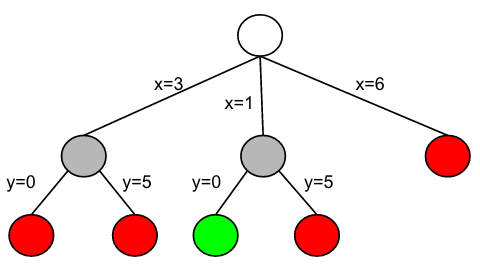
\includegraphics[width=4cm, height=2.4cm]{images/halfsearch.png}
% \end{minipage}
\begin{minipage}{.5\textwidth}
\centering
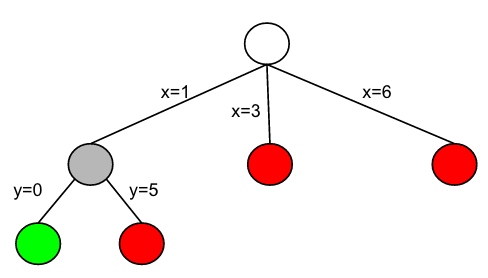
\includegraphics[width=3.8cm, height=2.4cm]{images/smallsearch.png}
\end{minipage}
\caption{All subproblems for $\pi$ checked by a branch and bound procedure with two different branching rules.}
\label{fig:bandb}
\end{figure}
\end{example}

As shown in Example \ref{ex:bandb}, the choice of bounding and branching procedures is crucial to the size of the explored search space. Existing literature has spent substantial effort in constructing efficient algorithms for branching and bounding \citep{Little63,Dantzig54, HeldK70}. Examples of such algorithms are discussed throughout this work for the studied NP-hard problems.

%\citet{Christofides81} say that ``... one of the most successful methods of solving routing problems is by the use of branch and bound algorithms where the effectiveness of the bounds is the most important parameter that determines the efficiency of the complete algorithm.'' There are different methods for computing bounds, some of which are discussed in this work (the AP relaxation, the set-partitioning model, etc.)

Branch and bound algorithms are one of the most successful methods for solving optimisation problems \citep{Christofides81} and they are typically implemented in Constraints Programming (CP) and Integer Programming (IP) solvers \citep{Leyffer01,Quesada92}.

\subsection{Linear and Integer Programming}
\label{ip}

Linear Programming (LP) is a way to solve problems by modeling their requirements as a system of linear inequalities and equations and subject to them finding an optimal solution to the problem, expressed as a function that has to be either minimised or maximised. This function is called the \textit{objective function}.

The field of LP is well-studied \citep{Kantorovich60,DantzigLp63} and it has many applications in the industry for resource optimisation \citep{Jacovkis89,Garvin57}. However, \citet{Dantzig60} shows that there are many important optimisation problems that can not be modeled as a linear program, because their variables can take only integer values. Such problems can be modeled with the tools of integer programming (IP). Integer programming (IP) is an extension of linear programming (LP). The difference between LP and IP is that in the IP model variables are restricted to take only integer values.

The rest of this section presents different methods to solve problems with the tools offered by IP and comments on their performance by using TSP as an example problem.

\subsubsection{Integer Programming Formulation of TSP}
% \texorpdfstring{TSP-$\Delta$}{Lg}}
\label{sec:iptspformulation}

\citet{Dantzig54} formulate TSP as the following IP problem. Let $x(i,j)$ be a variable that denotes whether city $j$ succeeds city $i$ in a TSP tour. The value of $x(i,j)$ is equal to 1 if this is true, or 0 if it is false. If $x(i,j)$ is 1, then $i$ is called the \textit{outgoing} city and $j$ - the \textit{incoming} city. The objective function of TSP is to minimise the total length of the tour, that is:

\begin{equation}
\label{eq:objfunc}
\textrm{min } \sum_{i\in A}\sum_{j\in A} d(i,j)x(i,j)
\end{equation}

In each TSP tour every city is visited once. Moreover, each city has to be incoming and outgoing exactly once. Therefore, the value of $x(i,j)$ for every $i$ will be 1 for only one $j$ and 0 for the rest. This can be enforced with the following constraint:

\begin{equation}
\label{eq:one}
\begin{split}
  \sum_{j \in A} x(i,j) = 1, \qquad i \in A,\\
  \sum_{i \in A} x(i,j) = 1, \qquad j \in A,
\end{split}
\end{equation}

Constraint (\ref{eq:one}) ensures that each city in $A$ is picked exactly once as an incoming and an outgoing city. However, it allows for the existence of one or more cycles of $n_{1} < n$ cities, called \textit{subtours}. For instance, consider Figure \ref{fig:tour} and Figure \ref{fig:subtours}. Both of them satisfy constraint (\ref{eq:one}). However, Figure \ref{fig:subtours} does not represent a valid tour, because it contains two subtours, each of size 3. To tackle this problem, \citet{Dantzig54} introduce the \textit{subtour elimination} constraint, that is:

\begin{equation}
\label{eq:subtourElimination}
\sum \{x(i,j) : (i,j) \in (S \times \bar{S}) \cup (\bar{S} \times S)\} \geq 2, \quad \forall \, \emptyset \subset S \subset A, \textrm{ where } \bar{S} = A \setminus S
\end{equation}

Here, $S$ is a subset of A and $\bar{S}$ is the set of all cities that are in $A$ and not in $S$. Constraint (\ref{eq:subtourElimination}) enforces that at least two cities in $S$ are connected with cities from $\bar{S}$. We give Figure \ref{fig:tour} and Figure \ref{fig:subtours} as an example. Let $S = \{A_{1},A_{2},A_{3}\}$, then $\bar{S} = \{A_{4},A_{5},A_{6}\}$. Constraint (\ref{eq:subtourElimination}), would detect the tour on Figure \ref{fig:subtours} as invalid, as there is no city in $S$ that is connected to a city in $\bar{S}$. Figure \ref{fig:tour} will be accepted, since $A_{1}$ and $A_{3}$ are connected with $A_{6}$ and $A_{4}$ respectively.

\begin{figure}
\centering
\begin{minipage}{.5\textwidth}
  \centering
  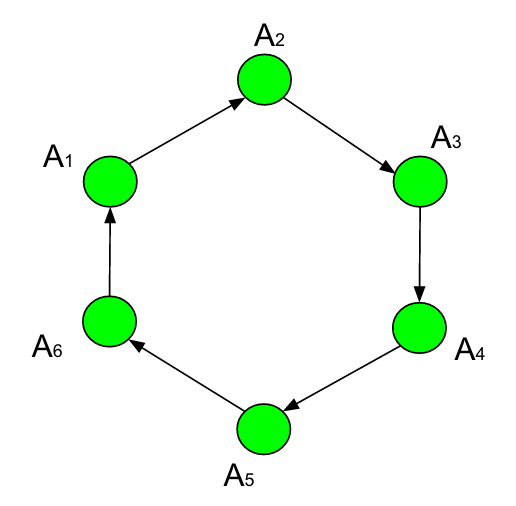
\includegraphics[width=4cm, height=4cm]{images/valid.png}
  \caption{A valid TSP tour}
  \label{fig:tour}
\end{minipage}%
\begin{minipage}{.5\textwidth}
  \centering
  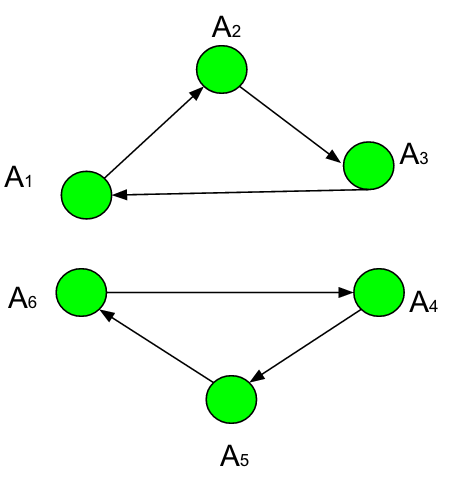
\includegraphics[width=4cm, height=4cm]{images/invalid.png}
  \caption{Two subtours of size 3}
  \label{fig:subtours}
\end{minipage}
\end{figure}

The formulation of the general TSP problem is given by the objective function (\ref{eq:objfunc}), which has to be minimised, subject to constraints (\ref{eq:one}) and (\ref{eq:subtourElimination}).

\subsubsection{The Assignment Problem Relaxation}
%The Assignment Problem (AP), formulated in Section \ref{npcompleteproblems}, can be represented with the tools of linear programming and it can be solved in at most $\mathcal{O}(n^{3})$ steps \citep{Kuhn55}. 

The assignment problem (AP) relaxation consists of removing the subtour elimination constraint from the TSP IP model and minimising the objective function (\ref{eq:objfunc}) only subject to constraint (\ref{eq:one}). This is well known and extensively used relaxation \cite{Fischetti92,Jonker80,Eastman58,Laporte86}. In this section we explain how this method helps in solving NP-hard problems, using TSP as an example.

Let $\pi^{\star}$ be the resulting problem after performing AP relaxation on some instance $\pi$ of TSP. 
The feasible solutions in $\pi$ correspond to travelling salesman tours and we let $opt(\pi)$ denote an optimal solution. The feasible solutions in $\pi^{\star}$ correspond to perfect matchings and we let $opt(\pi^{\star})$ correspond to a perfect matching of minimum weight.

Problem $\pi^{\star}$ can be modelled as a bipartite graph $G(V,E)$, as shown on Figure \ref{fig:tspbipartite}. The vertex set of $G$ is $V=O \cup I$, where $O = o_{1},..,o_{n}$ and $I = i_{1},...,i_{n}$ both correspond to $A$. The set of edges is $E = \{(o_{p}, i_{q}) \,|\, a_{p},a_{q} \in A,\, p \neq q \}$. Each edge $e = (o_{p}, i_{q}) \in E$ has weight $w_{e}$ equal to $d(a_{p},a_{q})$ and it represents a link from $a_{p}$ to $a_{q}$.

Figure \ref{fig:validAP} and Figure \ref{fig:invalidAP} are both examples of a perfect matching, where Figure \ref{fig:validAP} has $(o_{1} \rightarrow i_{2})$, $(o_{2} \rightarrow i_{3})$, $(o_{3} \rightarrow i_{4})$, $(o_{4} \rightarrow i_{5})$, $(o_{5} \rightarrow i_{6})$ and $(o_{6} \rightarrow i_{1})$.
Every $sol(\pi^{\star})$ can be translated to a path through the cities in $\pi$ as follows: for every matched pair of vertices $(o_{p} \rightarrow i_{q})$ in $sol(\pi^{\star})$, it is sufficient to choose city $a_{q}$ as the next visited city after $a_{p}$ in $\pi$. For example, the matching in Figure \ref{fig:validAP} gives the tour shown in Figure \ref{fig:tour} and the matching in Figure \ref{fig:invalidAP} is equivalent to the subtours in Figure \ref{fig:subtours}.

\begin{figure}
\centering
\begin{minipage}{.5\textwidth}
\centering
 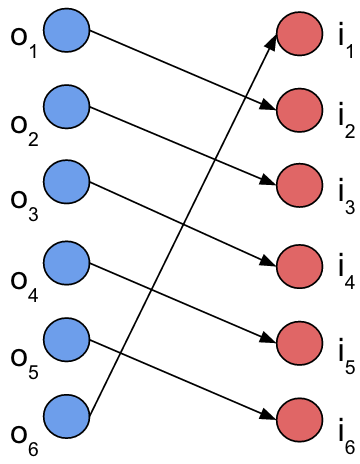
\includegraphics[width=3cm, height=4cm]{images/validAP.png}
 \caption{AP solution equivalent to Figure \ref{fig:tour}}
 \label{fig:validAP}
\end{minipage}%
\begin{minipage}{.5\textwidth}
\centering
 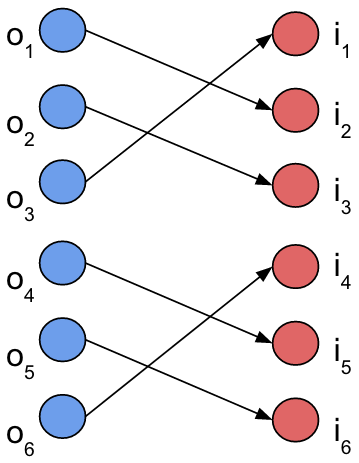
\includegraphics[width=3cm, height=4cm]{images/invalidAP.png}
 \caption{AP solution equivalent to Figure \ref{fig:subtours}}
 \label{fig:invalidAP}
\end{minipage}
\end{figure}

\begin{figure}
\centering
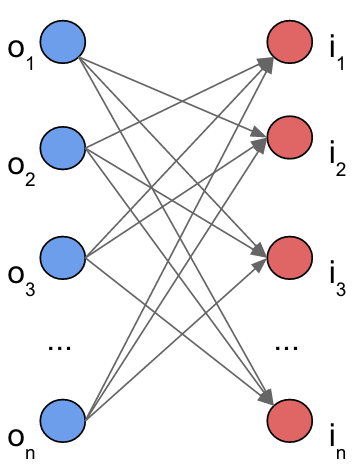
\includegraphics[width = 3cm, height = 4cm]{images/tspbipartite.png}
\caption{Problem $\pi^{\star}$ represented as a graph $G(V,E)$}
\label{fig:tspbipartite}
\end{figure}

Note that a feasible solution in $\pi$ maps to a feasible solution in $\pi^{\star}$, but the converse need not be true in general, as the example in Figure \ref{fig:invalidAP} shows.

Let $opt(\pi^{\star})$ have total edge weight equal to $\alpha$. Suppose that $opt(\pi^{\star})$ does not map to a tour in $\pi$. Therefore, $opt(\pi)$ must have length at least $\alpha$. Conversely, suppose that $opt(\pi^{\star})$ can be mapped to $opt(\pi)$. Therefore, the length of $opt(\pi)$ is equal to $\alpha$. Hence, the length of $opt(\pi)$ is greater than or equal to the value of $opt(\pi^{\star})$.
In the existing work, this property is used to derive a lower bound on the cost of $opt(\pi)$ \citep{Jonker80,Dantzig54,Dantzig59}. This approach is frequently combined with a branch and bound technique \citep{tspbible}, which is discussed in Section \ref{branchandbound}.

%\textcolor{blue}{The relation between TSP and AP is explained very nicely by \citet{Flood56}}

% \textcolor{red}{
% Another method for solving TSP with the AP relaxation is as follows. First, solve $\pi^{\prime}$. Then, check whether the solution contains any subtours and if yes, eliminate them. Iterate until a feasible enough solution is reached.}

% By dropping constraint (\ref{eq:subtourElimination}), the solution of $P_{AP}$ can be either a tour, or a collection of subtours. Hence, every tour of $P$ is a solution to AP, but not all solutions of AP are tours \citep{Bellmore71}. This allows for using the cost of the optimal solution of AP as a lower bound for the most optimal solution of $P$. In \cite{tspbible} it is showed with an experiment that both in theory and in practice the most optimal solution to AP is very likely to be a strong bound on $P$. The AP can be solved in at most $\mathcal{O}(n^{3})$ steps \citep{Kuhn55,Christofides75}. The ``bound'' procedure, that is called for every problem $P_{ij}$ in Algorithm \ref{alg:branchandbound}, computes AP$_{ij}$. It is shown in \cite{tspbible} that computing AP$_{ij}$ for each problem $P_{ij}$ in at most $\mathcal{O}(n^{2})$ steps by the Hungarian method \citep{Kuhn55}, provided that the algorithm is started from the optimal solution of the parent problem $P_{i}$.

\citet{Dantzig54} solve the constructed TSP model using a novel method for that time, which they call the ``cutting-plane method''. We point the interested reader back to \citep{Dantzig54} and \citep{Dantzig59}, where in the latter the cutting-plane method is explained in more detail using a 10 city TSP instance as an example.

The number of solved instances using the AP relaxation varies. \citet{Dantzig54} executes the algorithm by hand on a 49 city problem instance and there is no data on the computational performance of the algorithm. \citet{Jonker80} report on experiments with up to 150 city instances solved. However, the algorithm's running time is not specified. The greatest number of cities solved by \citet{Fischetti92} is 200. The longest time taken to solve a 200 city instance is 4.42 seconds, using a VAX 11/780 computer architecture.

% \textcolor{red}{
% \citet{Applegate03} implements a modification of the AP relaxation into Concorde \citep{concorde}, which is a TSP Solver that implements a variety of other techniques and heuristics. It ``is widely regarded as the fastest TSP solver, for large instances, currently in existence.'' \citep{Mulder03}. Concorde is capable of finding a feasible tour for instances with 1,000,000 cities or more \citep{Applegate03}.}

% what concorde can solve: \citep{concordeBenchmarks}
% tsp benchmarks: http://www.iwr.uni-heidelberg.de/groups/comopt/software/TSPLIB95/STSP.html

\subsection{Constraint Programming}
\label{cp}

Constraint Programming (CP) is a widely used method for solving optimisation problems \citep{Caseau97, Manlove07, Mcdonald02}. Given an instance $\pi$ of an optimisation problem, we first model it as a constraint satisfaction problem (CSP) $CSP(\pi)$. Problem $CSP(\pi)$ consists of a set of decision variables $V$, each with a set of possible values, called its \textit{domain}, and a set of rules, called \textit{constraints} concerning the assignment of domain values to variables. A \textit{solution} to $\pi$ is an assignment of each variable in $V$ to a value in its domain, such that all constraints are satisfied. The program that searches for a solution $CSP(\pi)$ is called a \textit{solver}.

Whenever the domain $dom_{v}$ of a variable $v$ is empty in some temporal assignment of variables, we say that we have a \textit{domain wipeout} and this variable's assignment is regarded as invalid. The \textit{degree} of $v$ is the number of constraints that involve $v$ and at least one other unassigned variable.

% todo: add citations
Finding a solution to $CSP(\pi)$ involves a search through the assignments of the variables in $CSP(\pi)$. Finding an optimal solution or proving that no solution exists requires iterating over the entire search space in the worst case. There are multiple techniques to speed up the search, such as identifying and discarding poor temporal variable assignments from further investigation, implementing intelligent search methods, or adding \textit{heuristics} for variable and value assignments. We discuss some heuristics that could be applicable to TP in the next section.

\subsubsection{Heuristics}
Heuristics are rules concerning the ordering of variables or assignments of values, used to ``guide'' the search, that aim to limit the total explored search space. Previous work has shown that heuristics can have a significant effect on search effort \citep{Haralick80:a, Gent96}. However, they are not guaranteed to always work. Heuristics are applicable for the cases when the solution is not required to be an optimum and when the particular problem instance has no solutions. In the latter, heuristics can help to prove early in the search that a given partial solution leads to a domain wipeout. This section presents some of the most well-known heuristics and gives an example of two successful heuristics that are tailored specifically for the Job-Shop Scheduling Problem (JSSP), defined in Section \ref{npcompleteproblems}.

Research effort is spent on understanding heuristics and the properties that improve their effectiveness. \citet{Christopher03} develop a framework for analysing the effectiveness of  heuristics. \citet{Hooker95} prove that heuristics that create simpler subproblems are successful in general, and heuristics that create subproblems that are more likely to be satisfiable are usually ``bad''. \citet{Haralick80} propose the intuition that ``to succeed, try first where you are most likely to fail'', known as the \textit{fail-first principle}. It suggests that the variable to be assigned next should be the one which is most-likely to lead to a domain wipeout of some variable.

The fail-first principle is a basis for the development of various heuristics. For instance, \citet{Golomb65} propose a heuristic \texttt{dom} that chooses next assigned variable to be the one with the smallest number of values remaining in its domain. \citet{Brelaz79} introduce a new generalisation of \texttt{dom}, denoted as \texttt{dom+deg}, which chooses the variable with the smallest number of values remaining in its domain, breaking ties on highest variable degree. Another generalisation of \texttt{dom} is \texttt{dom/deg}, which divides the domain size of a variable by the degree by its degree and chooses the variable that gives minimal value \citep{Bessiere96}. All of these are \textit{variable ordering} heuristics, because they determine the next explored variable during search.

%\textcolor{blue}{few words about how good fail-first principle is}

%\textcolor{blue}{Value-ordering heuristics examples}

% todo: explain why TP is similar to JSSP, why TP is similar to TSP. Maybe put the explanation in the problems definition.
\subsubsection*{Slack-Based Heuristics}

Slack-based heuristics were introduced by \citet{Smith93} for the JSSP, defined in Section \ref{npcompleteproblems}. They help in determining how to sequence a given pair of operations in an instance of JSSP, modelled as CSP. There are various ways to model JSSP as CSP, which is a significant area of research on its own. We refer the interested reader to \citet[Chapter~22]{cpbible} for an extensive discussion.
This section explains the main principles of the slack-based heuristics, comments on their performance and discusses our hypothesis that it could be applicable to TP (which is the main reason why they are discussed here).

Let $\pi_{J}$ be an instance of the JSSP and let $CSP(\pi_{J})$ be constructed using some CSP model for JSSP, which includes a variable $o(i,j)$ that determines the ordering of any pair of operations $i$ and $j$ in $\pi_{J}$. The value of $o(i,j)$ is 1 when $i$ is scheduled before $j$, or 0 otherwise. There are four possible restrictions for the values of $o(i,j)$, imposed by the constraints in $CSP(\pi_{J})$:

\begin{enumerate}
\item $o(i,j)$ can only be 1, i.e. $i$ is before $j$ in the current variable assignment.
\item $o(i,j)$ can only be 0, i.e. $j$ is before $i$ in the current variable assignment.
\item $o(i,j)$ can be neither 0 nor 1, i.e. there is a domain wipeout.
\item $o(i,j)$ can be either 0 or 1, i.e. there is no restriction on the ordering of $i$ and $j$.
\end{enumerate}
Slack-based heuristics are only applicable for case 4 and thus we skip discussion of the first three possibilities.

For every $o(i,j)$ that can be either 0 or 1, \citet{Smith93} compute $slack(i, j)$, which is the time remaining after ordering $i$ before $j$ and similarly $slack(j, i)$, as shown by the pink bars in Figure \ref{fig:slack}. If process $i$ is sequenced before process $j$, then $slack(i, j)$ indicates the time window within which $j$ has to be completed.
Two different heuristics for the sequencing of $i$ and $j$, based on the size of the time window are introduced: \textit{min-slack} and \textit{max-slack}.

\begin{figure}[H]
\centering
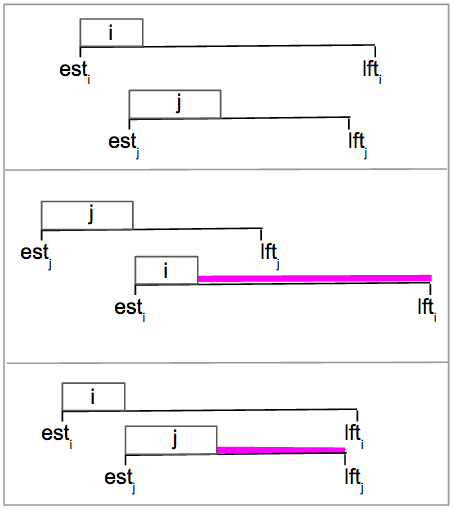
\includegraphics[height=7cm, width=6cm]{images/slack.png}
\caption{The values of $slack(i, j)$ (the length of the bottom pink line) and $slack(j, i)$ (the length of the top pink line), where $est_{x}$ and $lft_{x}$ refer to the earliest start and finish time of an operation $x$ respectively.}
\label{fig:slack}
\end{figure}

Min-slack ordering selects an ordering of $i$ and $j$ that gives minimum time flexibility for the tasks. For instance, min-slack heuristics would assign $o(i,j) = 1$ for the example in Figure \ref{fig:slack}.
Max-slack heuristic orders the operations, such that there is greatest time flexibility for the tasks. In the example in Figure \ref{fig:slack}, max-slack would assign $o(i,j) = 0$, since $slack(j, i) > slack(i, j)$.

We relate the idea behind min-slack to the principles of the \texttt{dom} heuristic. If the starting times of $i$ and $j$ are variables, then the assignment of $o(i,j)$ based on min-slack would decrease the domain of the starting time of the second scheduled process. As opposed to min-slack, max-slack would maximize the number of possible starting times. We recognise that this idea can be traced back to the work of \citet{Geelen92} which proposes a principle that each variable should be assigned the least constraining value in its domain.

\citet{Smith93} compare the slack-based heuristics with two solution procedures over the same suite of benchmark problems and report on obtaining ``comparable results at very low computational expense''. In \citet[p.~105]{cpbible}, slack-based heuristics are described as ``effective''. However, \citet{Crawford94} argue that their effectiveness is mainly due to their problem representation method.

\subsection{Algorithms for the Time-Constrained TSP}
\label{sec:tctspalgos}
Time-Constraint TSP (TCTSP), also known as TSP with Time Windows (TSPTW) is a generalisation of TSP, defined in Section \ref{npcompleteproblems}.
Although there is a substantial amount of work done on TCTSP, most of the attention in the literature seems to be for TSP \citep{tspbible} and many techniques for TCTSP are TSP models, adapted to include time windows constraints. This section is a discussion of common approaches to model and solve TCTSP.

%% todo: briefly introduce the dual model here
\citet{tspbible} present a summary of the most used techniques to model TCTSP. One of them is similar to the TSP IP formulation in Section \ref{sec:iptspformulation}, having each of the variables adapted to consider specific time periods. \citet{tspbible} also discuss the dual model introduced by \citet{Baker83} as an example of an effective technique.

%%% todo: explain more about the longest path algorithm
\citet{Baker83} works with instances with symmetric inter city distances under the triangle inequality. TCTSP is modelled as a system of linear integer inequalities, solved by a branch and bound procedure with bounds calculated using an algorithm for the longest path problem \footnote{The longest path problem is the problem of finding a path of maximum length in a graph with no repeated vertices.}.

% \subsubsection{The dual model for TCTSP}
% \label{sec:baker83}

% \textcolor{red}{The dual model for TCTSP is introduced by \citet{Baker83} and it is referred to as ``the most elegant'' method to model TCTSP \citep{Chan05}. It consists of a system of linear integer inequalities that yields a disjunctive graph, known from scheduling theory \citep{Baker83}. The solution implements a branch and bound procedure with bounds calculated using the longest path algorithm. Baker's algorithm works for instances with symmetric inter city distances under the triangle inequality, where the distance between two cities $i$ and $j$ is \textit{symmetric} if $d(i, j) = d(j, i)$. Moreover, if the traveller arrives at city $i$ at time $t_{i} < l_{i}$, she is allowed to wait until the $t_{i} = l_{i}$ and the time window opens.}

% \textcolor{red}{The term \textit{time window} for a city $i$ refers to the period of time between $l_{i}$ and $u_{i}$ in which $i$ has to be visited. \citet{Baker83} introduces a variable $t_{i}$ for each city $i$ that determines the time $i$ is visited in the tour and an additional variable $t_{n+1}$ that determines the time at which the tour is completed. The objective function of the problem is:}

% \textcolor{red}{This model allows for the traveller to arrive at city $i$ at time $t_{i} < l_{i}$, provided that she waits in $i$ until the time window opens. Moreover, although a single upper and lower bound on the time window is assumed, the model could be easily extended to include sets of distinct time windows for each city \citep{Baker83}.}

% \textcolor{red}{The objective function of the model indirectly imposes the constraint that the number of visits to each city has to be one. Suppose the TCTSP algorithm returned a tour containing city $i$ more than once. Then the tour would not be optimal, because one could do better by cutting one of the visits to $i$ until $i$ is visited only once \footnote{This is true, since the distances are under the triangle inequality and the traveller is allowed to arrive at a city before the start of the time window, provided that she waits until it opens.}.}

% \textcolor{red}{
% A \textit{disjunctive graph} is a way of modelling a system of tasks to be scheduled within certain time constraints, introduced mainly for scheduling problems \citep{tspbible}. For TCTSP, this is a graph $G=(V,E,A)$, where the set of vertices $V$ represents all cities in the problem, $E$ is the set of undirected edges and $A$ is the set of directed edges. For every two vertices $i$ and $j$, $e(i,j) \in E$ if and only if cities $i$ and $j$ can be visited in either order, in which case they have \textit{disjunctive} relation, and $e(i,j) \in A$ if and only if $i$ must be visited before $j$. Constraint (11) represents two discrete cases and thus yields the disjunctive relations between cities.}

% \textcolor{red}{Using previously shown relation between TSP and the longest path problem \citep{Hardgrave62}, \citet{Baker83} relaxes constraints (11) and (14) and shows that the resulting relaxed problem $P$ is equivalent to the longest path problem \footnote{The longest path problem asks to find a path of maximum length in a given graph.}. Although this problem is also NP-hard, it is hoped that it is easier than TSP \citep{Hardgrave62}.}

% \textcolor{red}{
% The bounding procedure of the branch and bound algorithm consists of finding the longest path in every relaxed subproblem. For every non-discarded subproblem, the additional cases from constraint (11) are added.
% \citet{Baker83} enforces constraint (14) by adding dual labelling on the vertices in the disjunctive graph within the branch and bound procedure. The first label of a vertex $v$ that represents city $i$ is $i$ and the second label of 
% $v$ is the value $p_{i}$ of the longest path from vertex 1 to $i$. If $p_{i} > u_{i}$, then the current assignment of values to variables gives no solution. If $p_{i} < l_{i}$, then the traveller has to wait at $i$ until the time window opens. Thus, the value of $p_{i}$ is $t_{i}$.}

% \textcolor{red}{\citet{Baker83} conduct experiments using 20 problem instances of size 9, 13, 22, 30 or 51 cities with varying percent of overlapping windows.
% The experiments show that this approach is effective on small to moderate-sized instances and that its efficiency greatly depends on the number of overlapping time windows. For each set of instances with equal city size, the problem that took most CPU time is the one with least number of overlapping windows. For the 51 city problem the program did not terminate for this instance.
% Therefore, TCTSP instances with greater number of overlapping time windows are easier to solve. We conjecture that the reason for this could be that the model is more constrained and therefore the number of possible subproblems that have to be checked during the branch and bound procedure is smaller.}

\citet{Baker83} conducts experiments using 20 problem instances of size 9, 13, 22, 30 or 51 cities with varying percent of overlapping windows.

\citet{ariglianotime} work on TCTSP with asymmetric distances 
and construct an integer linear programming model using a variation of the cutting planes algorithm. The paper argues that a limitation of existing TCTSP algorithms such as \citep{Baker83} is that they assume that the travel time is constant. \citet{ariglianotime} make TCTSP seem more related to real-world problems by introducing the notion of \textit{travel speed}, \textit{congestion factor} and \textit{travel time}, where the latter is a function of the former two variables. \citet{ariglianotime} can solve instances with up to 40 cities.

\citet{Hurkala15} is a recent work that is believed to be the first to consider problems with multiple time windows. The paper agrees with \citet{ariglianotime} that the constant travel time assumption is unrealistic and the TCTSP model is also adapted to changing travel times. \citet{Hurkala15} introduces a novel algorithm for this re-formulation of TCTSP and combines it with three already existing metaheuristics to produce three TCTSP solvers. For the empirical evaluation, \citet{Hurkala15} uses 45 randomly generated instances with 13 to 23 cities, which is almost twice as small as the maximum number of cities that \citet{ariglianotime} can solve. This suggests that multiple time windows add additional complexity to the problem.

\subsection{Algorithms for the Time-Constrained Vehicle Routing Problem}
\label{sec:tcvrpalgos}
This section outlines the main approaches to the Time-Constrained Vehicle Routing Problem (TCVRP), often known as the Vehicle Routing Problem with Time Windows (VRPTW). TCVRP is a generalisation of TSP and it is defined in Section \ref{npcompleteproblems}.

A common approach in the literature is to model VRP and TCVRP as a \textit{set partitioning problem} \citep{Desrochers92,Agarwal89,Desrosiers84,Alvarenga07}. This can be done as follows. Let $\mathcal{R}$ be the set of all feasible routes, where $c_{r}$ denotes the cost of a route $r \in R$. Let $\delta_{i,r}$ and $x_{r}$ be two variables that can be either 0 or 1. For each $r \in R$, $\delta_{i,r}$ is 1 if $r$ visits city $i$ and $x_{r}$ is 1 if $r$ is used in the solution. Then, TCVRP can be formulated as the problem of choosing a set $\mathcal{S} \subset R$ with minimal cost, known as the \textit{set partitioning problem} (SPP), that is:

\begin{equation}
\label{eq:tcvrpobjfunc}
\textrm{minimise } \sum_{r \in R} c_{r} x_{r},
\end{equation}

\begin{equation}
\label{eq:tcvrpconstraint1}
\sum_{r \in R} \delta_{i,r} x_{r} = 1, \quad \forall i \in A \setminus \{D\},
\end{equation}

where constraint (16) imposes that each city is part of a set which is used in the solution. Some algorithms then construct a LP relaxation of this formulation and use the solution of the relaxation as a lower bound for a specific branch and bound procedure \citep{Desrochers92,Agarwal89}.

The method outlined above is somewhat similar to the AP LP relaxation for TSP. This shows that this general approach, dating back to the work of \citet{Dantzig54}, is highly applicable to different NP-hard problems.

Some approaches are based on heuristics \citep{Tan99heuristicmethods,Cheng09}. \citet{Braysy05,Braysy05a} show the importance of good heuristics for tackling TCVRP. They present a review of some route construction and route improvement heuristics and attempt to outline a guideline for the evaluation of heuristics.
For more detailed review, we refer the interested reader further to \citet{Toth14}, where the practical aspects of TCVRP are discussed and common methods to solve TCVRP as well as some of its other variations are outlined.

The number of cites in a solved instance varies across the different algorithms. For the algorithms based on the set partitioning model, \citet{Agarwal89} solve instances with up to 25 cities in their computational experiments. \citet{Desrosiers84} work with real-world bus transportation problems and they solve instances with up to 55 schools, where schools are equivalent to cities. \citet{Desrochers92} is the first work capable of optimally solving instances with 100 cities. They say that ``... this problem size is six times larger than any reported to date by other published research.''
Heuristics-based approaches can also find solutions to instances with up to 100 cities \citep{Tan99heuristicmethods}. However, one should note that these solutions need not be optimal.

% \subsection{Multiobjective Optimisation}
% Multiobjective optimisation problems have more than one objective function to be optimised simultaneously. For instance, adding the soft constraints in Section \ref{subsec:softconstraints} to the TP formulation would give a multiobjective optimisation problem.
%In such case, a weighting factor is assigned to each objective and the problem is to optimise the new objective function, obtained by summing all objectives, with each of them multiplied by its weighting factor. In this Section, we briefly discuss existing approaches to multiobjective optimisation.

\subsection{Summary}

This section outlines the main observations from the literature survey and shows their influence on the proposed approach in Section \ref{sec:proposedapproach}.

Most of the existing approaches to NP-hard problems generally follow a similar pattern. For instance, this can be a relaxation to another problem which need not be polynomial-time solvable in order to obtain a lower bound on the solution, used as part of a branch and bound procedure. Many algorithms model the problem as a constraint satisfaction problem or as a system of linear integer inequalities.

The average size of TSP instances tackled by existing algorithms outweighs the size of the solvable instances of the other studied problems, namely VRP, TCTSP and TCVRP for which TSP is a special case. TCVRP is a generalisation of each of TSP, VRP and TCTSP and it is the problem with smallest maximum size of solved instances by the existing literature. This observation is later used in Section \ref{sec:evaluation} when deciding on feasible sizes of the datasets.

When it is not necessarily vital that a given instance of TP is solved to optimality, there are algorithms that can return their ``best'' solution found so far after a given period of time. CP or IP solvers for instance offer this flexibility. Typically, much larger instances can be solved, since in many cases the algorithm does not need to explore the entire search space to prove the optimality of a solution, that may have been found relatively early on in search (and which itself may even be optimal). This will be investigated during the project evaluation.

% \textcolor{red}{
% In Section \ref{cp} we gave examples of many successful heuristics for minimising the size of variables' domains. Therefore, the fact that TP has multiple constraints could mean that the larger size of solvable TP instances, compared to other studied problems.  In Section \ref{sec:evaluationgoals} we explain our predictions, noting that the size of a TP instance can vary with respect to multiple entities and that a feasible solution often need not be an optimal solution.} \textcolor{blue}{Obtaining a good }

%%%%%%%%%%%%%%%%%%%%%%%%%%%%%%%%%%%%%%%%%%%%%%%%%%%%%%%%%%%%%%%%%%%

\section{Project Requirements}
\label{sec:requirements}

\begin{figure}
\centering
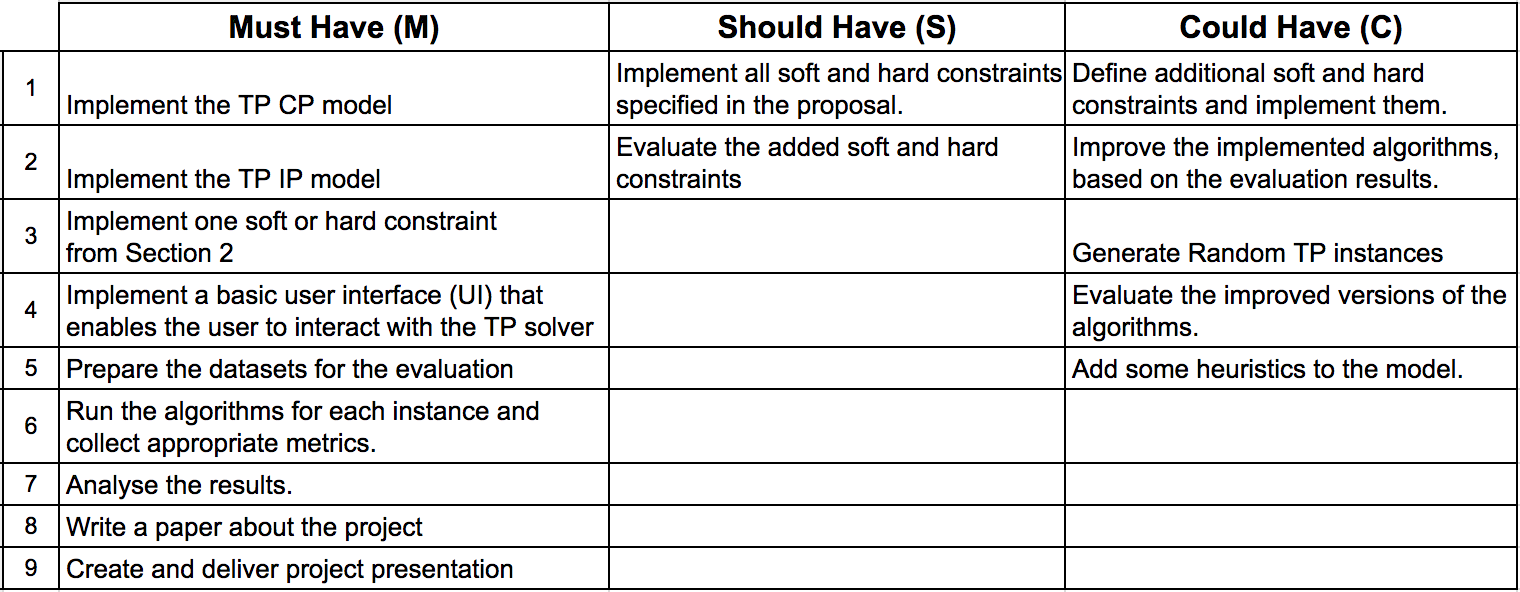
\includegraphics[width = 16cm, height = 6 cm]{images/requirements.png}
\caption{Project requirements.}
\label{fig:requirements}
\end{figure}

%%% do I need to write how I captured these requirements?
This section lists the project requirements. They are separated into three categories: must have, should have and could have, based on the MoSCoW technique for requirements prioritization \citep{ash2007moscow}. Requirements under the \textit{must have} category are critical to the success of the project. \textit{Should have} requirements are important, but not necessary for the successful completion of the project. \textit{Could have} requirements are desirable, but not necessary and their purpose is to improve the overall quality of the project. Figure \ref{fig:requirements} shows all project requirements. To refer to a specific requirement we use its \textit{id}, which is the string composed of the first letter of the requirement category (M, S or C) and the number of the row the requirement is in. For instance, requirement ``Define additional soft and hard constraints and implement them'' has id $C1$. This list is later referred to in Section \ref{sec:workplan} where we describe the work plan.

% \begin{table}
% \centering
% \renewcommand{\arraystretch}{1.4}% Spread rows out...
% \begin{tabular}{c|r|r|r|}
% \cline{2-4}
% & 
% \multicolumn{1}{|c|}{\textbf{Must Have (M)}} & 
% \multicolumn{1}{|c|}{\textbf{Should Have (S)}} & 
% \multicolumn{1}{|c|}{\textbf{Could Have (C)}} \\
% \cline{2-4}
% \hline
% \multicolumn{1}{|l|}{\textbf{1}}  &Implement the TP CP model &Implement the TP IP model &\specialcell[t]{Improve the UI } \\
% \multicolumn{1}{|l|}{\textbf{2}}  &20,816 & 4 &592 \\
% \multicolumn{1}{|l|}{\textbf{3}} &219,184 &91.33 & 55 \\
% \multicolumn{1}{|l|}{\textbf{4}} &219,184 &91.33 & 55 \\
% \multicolumn{1}{|l|}{\textbf{5}} &219,184 &91.33 & 55 \\
% \multicolumn{1}{|l|}{\textbf{6}} &219,184 &91.33 & 55 \\
% \multicolumn{1}{|l|}{\textbf{7}} &219,184 &91.33 & 55 \\
% \multicolumn{1}{|l|}{\textbf{8}} &219,184 &91.33 & 55 \\
% \hline
% \end{tabular}
% \caption{The number of SAT/UNSAT SIP instances for each dataset}
% \label{table:dataSAT}
% \end{table}


%%%%%%%%%%%%%%%%%%%%%%%%%%%%%%%%%%%%%%%%%%%%%%%%%%%%%%%%%%%%%%%%%%%
\section{Proposed Approach}
\label{sec:proposedapproach}
Based on the analysis of existing work in Section \ref{sec:existingwork}, we model TP as Integer and Constraint Programming problems. The Constraint Programming (CP) approach is explained in Section \ref{subsec:tpcp} and the Integer Programming (IP) model is presented in Section \ref{subsec:tpip}. Having two distinct TP models would allow for each of the models to be used as an additional verification step for the correctness of the other. Since optimal solutions of each TP instance have equal numeric value, if TP CP and TP IP return the same numeric value of an optimal solution for a large number of sufficiently-large instances, this will provide strong evidence that both models are correct. A difference in their solutions would indicate a mistake in either of them. Having more than one TP algorithm also gives opportunities for performing more detailed evaluation, learn more about the problem and about CP and IP.

\subsection{CP Model}
\label{subsec:tpcp}

Let $m = |F|$. We introduce an array $\mathcal{S}$ of size $m+1$ (indexed $0,1,...,m$) that represents the TP tour and a variable $z$ with domain $dom_{z} = \{1,...,m\}$ to denote the number of flights in the trip. If $\mathcal{S}[i] = j$, then flight $f_{j} \in F$ is the $(i+1)^{th}$ flight in the tour, for $(0 \leq i < m)$ and $(1 \leq j \leq m)$. To denote the end of the tour, we set $\mathcal{S}[z] = 0$. All subsequent variables in $\mathcal{S}$ will then have to be 0. Each variable $v$ in $\mathcal{S}$ is either 0, if no flight is taken at that step, or it is equal to some flight number, that is $dom_{v} = \{0,...,m\}$.

TP can then be formulated as the problem of minimising the objective function:

\begin{equation}
\label{eq:TPwithCPobj}
\sum^{m-1}_{i = 0} c_{\mathcal{S}[i]}
\end{equation}

subject to constraints (12-18).

\begin{itemize}
\Item
$\mathcal{S}[i] > 0 \wedge \mathcal{S}[i+1] = 0 , \quad (0 \leq i \leq z-1)$
\end{itemize}
\begin{itemize}
\Item
$\textrm{allDiff}(\mathcal{S}[0],...,\mathcal{S}[z-1])$
\end{itemize}

Constraint (12) restricts that once the end of the trip is reached at some position $z$, no flights are further added to $\mathcal{S}$. Constraint (13) enforces that every flight is taken only once, using an all-different constraint \citep{Hoeve01}.

The trip properties are added to the model as follows:

\begin{itemize}
% property 1:
\Item
$dom_{\mathcal{S}[0]} = \{j \in \{1,...,m\} : A^{d}_{j} = A_{0}\}$
\item[]
$dom_{\mathcal{S}[z-1]} = \{j \in \{1,...,m\} : A^{a}_{j} = A_{0}\}$
% property 2:
\Item
$dom_{\mathcal{S}[i]} = \{j \in \{1,...,m\} : A^{d}_{j} = A^{a}_{p}, \, p = \mathcal{S}[i-1]\}, \quad (1 \leq i < z)$
\end{itemize}

\begin{itemize}
% property 3:
\Item
$t_{p} + \Delta_{p} + C_{r} \leq t_{q}, \textrm{ where } p = \mathcal{S}[i], q = \mathcal{S}[i+1], r = A^{a}_{q}, \, (0 \leq i < z)$
\end{itemize}

\begin{itemize}
% property 4:
\Item
$t_{q} + \Delta_{q} \leq T, \quad \textrm{ where } q = \mathcal{S}[z-1]$
% property 5:
\Item
$\forall A_{k} \in D, \, |\{i: (0 \leq i < z) \wedge A^{a}_{\mathcal{S}[i]} = A_{k} \}| > 0 $
\end{itemize}

Constraint (14) is equivalent to trip property (1). It restricts the domains of the first and the $(z-1)^{th}$ variable in $\mathcal{S}$ to contain only flights that depart from/arrive at the home point. Trip property (2) is enforced by constraint (15). The domain of each variable in $\mathcal{S}$ is set to include only flights that depart from the arrival airport of the previous flight. Constraints (16) and (17) correspond to trip properties (3) and (4) respectively. Constraint (18) restricts that the number of the flights that arrive at every destination in the trip is positive, and thus enforces trip property (5).

\subsection{IP Model}
\label{subsec:tpip}

Most of the constraints for the TP CP model need modification in order to be applicable to an IP model. In particular, IP does not allow for ``if-then'', ``all-different'' and other constraints that are not integer linear inequalities. The model described in this section is a modification of the TP CP model, described in the previous section, that gives constraints in the form of integer linear inequalities, which we also refer to as \textit{ constraints}.

Let $m = |F|$. We introduce a variable $x_{i,j}$ for every $i \in \{0,...,m-1\}$ and  $j \in \{1,...,m\}$, such that $x_{i,j} = 1$ if $(i+1)^{th}$ flight is $f_{j}$ or 0 otherwise. This variable is somewhat similar to $\mathcal{S}$, used for the CP model, where $\mathcal{S}[i] = p$ is equivalent to $x_{i,p} = 1$. In addition, we introduce a variable $x_{m,0} = 1$, where flight $f_{0}$ is a ``special'' flight with duration $\Delta_{j} = 0$, date $t_{j} = T$, departure and arrival airports $A^{d}_{j} = A^{a}_{j} = A_{0}$ and cost $c_{j} = 0$, added to $F$. 


The objective function of TP is to minimise:

\begin{equation}
\label{eq:TPwithIPobj}
\sum^{m-1}_{i} \sum^{m}_{j=0} c_{j=1} x_{i,j}
\end{equation}

subject to constraints (20-26).

First, we restrict that only one flight is taken at each step $i$ with constraint (20). Constraint (21) is equivalent to the all-different constraint (13): it enforces every flight to be taken at most once.

\begin{itemize}
\Item
$\forall i \, (0 \leq i < m), \quad \sum^{m}_{j = 1}x_{i,j} = 1 $
\Item
$\forall j \, (0 \leq j \leq m), \quad \sum^{m-1}_{i = 0}x_{i,j} = 1 $
\end{itemize}

Our method to express the properties of a trip as integer linear inequalities is as follows. Assume that flight $z-1$ is the final flight returning to $A_{0}$, where $1 \leq z \leq m$. We add $m-z+1$ many $f_{0}$ flights, so that the variables $x_{z,0},...,x_{m,0}$ are all equal to 1. We do not add connection time when connecting from $A_{0}$ to $A_{0}$ as part of these flights.

Constraints (22) and (23) enforce trip property (1). The first flight is restricted to depart from the home point and the last flight must arrive at the home point.
From trip property (2) it follows that there must exist some $z < m$, $x_{z,j} = 1$, for which $j \neq 0$ and $A^{a}_{j} = A_{0}$. Thus, constraint (23) indirectly enforces that $A^{a}_{j} = A_{0}$.

\begin{itemize}
% property 1:
\Item
$\sum_{j \in S_{1}} x_{0,j} = 1, \quad \textrm{where } S_{1} = \{j \in \{1,...,m\} : A^{d}_{j} = A_{0}\}$
\Item
$x_{m,0} = 1$
\end{itemize}

Property (2) is enforced by defining two sets of flights $S_{1}$ and $S_{2}$, such that all flights in $S_{2}$ depart from the arrival airport of $S_{1}$. Constraint (26) restricts that every flight always departs from the arrival airport of the previous taken flight.

\begin{itemize}
% property 2:
\Item
$\sum_{j \in S_{1}} x_{i-1,j} = \sum_{j^{\prime} \in S_{2}} x_{i,j^{\prime}}, \quad \forall i \, (1 \leq i \leq m) \wedge \forall y \in A, \textrm{ where}$
\item[]
$S_{1} = \{j \in \{0,...,m\} : A^{a}_{j} = y\} \textrm{ and } S_{2} = \{j^{\prime} \in \{0,...,m\} : A^{d}_{j^{\prime}} = y\}$
\end{itemize}

Trip properties (3) and (4) are represented by constraint (31), which enforces that every flight $f_{j}$ cannot depart until the previous flight $f_{j^{\prime}}$ has arrived, adding connection time, if needed.% The connection time $C^{\prime}_{r}$ is equal to the connection time of the arrival airport, unless the current flight is $f_{0}$.

\begin{itemize}
% property 3 and 4:
\Item
$x_{i+1,j} + \sum_{j^{\prime} \in F^{\prime}} x_{i,j^{\prime}} \leq 1, \quad \forall i \, (0 \leq i < m) \textrm{ and }  \forall j \, (0 \leq j \leq m)$
\item[]
$\textrm{where } F^{\prime} = \{j^{\prime} : f_{j^{\prime}} \in F \wedge t_{j^{\prime}} + \Delta_{j^{\prime}} + C^{\prime}_{r} > t_{j} \} \textrm{ and}$
\item[]
$C^{\prime}_{r} =   \begin{cases}
0, \quad \textrm{ if } j=0 \\
C_{A^{a}_{j^{\prime}}}, \quad \textrm{ otherwise}
\end{cases}
$
\end{itemize}

% property 5:
Trip property (5) is enforced by restricting that all destination airports must be visited by at least one flight:

\begin{itemize}
\Item
$\forall A_{k} \in D, \, \sum_{i=0}^{m-1} \sum_{j \in F_{k}} x_{i,j} \geq 1, \quad \textrm{ where } F_{k}= \{j : f_{j}\in F \wedge A^{a}_{j} = A_{k}\} $
\end{itemize}

\subsection{Modelling soft and hard constraints}
\label{sec:modelsoftandhardconstr}

This section shows how soft and hard constraints in Section \ref{sec:tpformulation} can be added to the constructed models for TP, using hard constraint 2 in Section \ref{subsec:hardconstraints} as an example.

Let $U \subseteq D$ be the set of all destinations which must be visited at some specific date. The TP formulation allows for destination airports to be used as connections. Therefore, pruning all flights departing from or arriving at a constrained destination $A_{i}$ before or respectively after the required date $\tau_{i}$ for $A_{i}$ potentially removes feasible solutions. Instead, we add constraint (27) which ensures that for every destination $A_{i}$ in $U$, there is a scheduled flight arriving at $A_{i}$ before the required date $\tau_{i}$ and the next scheduled flight departs from $A_{i}$ after $\tau_{i}$.

\begin{itemize}
\Item
$\forall A_{i} \in U, \, \exists j \, (0 \leq j < z) \textrm{, such that:}  $
\item[]
$A^{a}_{\mathcal{S}[j]} = A_{i},$
\item[]
$t_{\mathcal{S}[j]} + \Delta_{\mathcal{S}[j]} + C_{i} < \tau_{i}, \textrm{ and}$
\item[]
$t_{\mathcal{S}[j+1]} > \tau_{i} + 1$ \footnote{We assume that the traveller has to stay at $A_{i}$ for at least one day after the required date $\tau_{i}$.}
\end{itemize}

Constraint (27) is defined as an addition to the CP model presented in Section \ref{subsec:tpcp}. Other required soft or hard constraints can be enforced using similar methods for either of the two models.

% \begin{itemize}
% \Item
% $\forall A_{i} \in U, \, \exists f_{p},f_{q} \in \mathcal{S} \textrm{ such that } \mathcal{S}[j] = f_{p} \wedge \mathcal{S}[j+1] = f_{q}  \textrm{ such that:}  $
% \item[]
% $A^{a}_{p} = A_{i} \wedge t_{p} + \Delta_{p} + C_{i} \leq \tau_{i} \wedge A^{d}_{q} = A_{i} \wedge t_{q} > \tau_{i}$
% \end{itemize}


%The method presented below is suited for the TP CP model and it is added as a filtering step before the construction of the model, specified in Section \ref{subsec:tpcp}. It prunes all flights that would make the solution invalid, if taken by the traveller.

% Let $\tau_{i}$ denote the date at which the traveller must be at destination $A_{i}$. Having $\tau_{i} = 0$ indicates that there is no such restriction for $A_{i}$ and $\tau_{i} \geq T$ implies that the TP instance has no solution.

% \begin{itemize}
% \Item
% $\forall A_{i} \in D \textrm{ such that } \tau_{i} \neq 0 \wedge \tau_{i} < T:$
% \item[]
% $\forall f_{j} \in F, \, A^{d}_{j} = A_{i} \wedge t_{j} < \tau_{i} \rightarrow F = F \setminus \{f_{j}\}$
% \item[]
% $\forall f_{j} \in F, \, A^{a}_{j} = A_{i} \wedge t_{j} > \tau_{i} \rightarrow F = F \setminus \{f_{j}\}$
% \end{itemize}

% Procedure (27) removes from $F$ all flight that make the traveller either arrive at the destination after the date constraint or leave the destination before the date constraint.

% Note that this approach does not allow for using destinations also as connection airports, thus it could produce flight schedules with higher price than the optimal.

\subsection{Choice of CP and IP solvers}
\label{sec:cpandisolvers}

We were unable to find a solver that supports both IP and CP and this is the reason why the TP IP and CP models will be implemented using two different solvers. In order to decrease the implementation difference between the two models as much as possible, we have chosen solvers that support the same language, namely  Java.

Choco \citep{choco} is an open-source Java library for Constraint Programming that has wide range of already implemented constraints and heuristics. One only states the variables and constraints and then the problem is solved using specific internally implemented search algorithms. The TP CP model will be implemented using Choco.

Gurobi is a mixed-integer programming solver first released in 2009. It is widely used mathematical optimisation tool \citep{gurobiusage} and it is licensed freely to academia. We will use Gurobi for the implementation of the TP IP model.

Both Gurobi and Choco are well-documented with good support from the community and easy to set up and use, which are the main reasons why we choose to use them.

\subsection{Evaluation}
\label{sec:evaluation}

This section is the plan of the project evaluation. The main goal of the evaluation is to analyse the implemented algorithms for TP and learn more about the problem and its extensions and variations. To achieve this, it is important to create instances that are good representatives of instances of TP that are likely to be encountered in practice and to measure appropriate metrics. 
Section \ref{sec:evaluationgoals} presents our choice of evaluation metrics and Section \ref{sec:datasets} gives more background on the experimental datasets.

\subsubsection{Evaluation Measurements}
\label{sec:evaluationgoals}

The main metrics that will be taken when running each of the algorithms are the following:
\begin{enumerate}
\item The number of \textit{search nodes} taken to solve each instance.
\item The running time of each of the algorithms for each instance.
\item The ``best'' returned solution when running for a given period of time and how far from an optimum it is.
\item The number of optimal solutions for each instance.
\item The number of airports, the number of destinations, the size of the flights set and the travel time period of the largest instances.
\end{enumerate}

The number of \textit{search nodes} denotes the number of recursive calls taken to find a solution if the problem is soluble or prove that the problem is insoluble. This metric is used by the existing literature to measure the hardness of an instance \citep{McCreesh16}.

For metric 3, we measure how far from an optimum the returned solution is by comparing it with an optimal solution, returned after running the exact TP algorithms. We plan to find optimal solutions with respect to the following objective functions:

\begin{itemize}
\item Minimise the sum of the cost of each flight;
\item Minimise the length of the flights schedule;
\item Minimise the number of airports taken as connections;
\item Minimise the time spent on flying;
\item Minimise the connection time;
\item Minimise a set of the aforementioned objectives. 
\end{itemize}

By collecting metrics 1 and 2, we aim to learn more about how the size of TP instances influences the behaviour of the implemented algorithms. Metric 3 measures the trade-off between computation time and optimality of a solution. Metric 4 shows some of the properties of the datasets. Metric 5 aims to show the properties of the largest solvable instance.

\subsubsection{Experimental Datasets}
\label{sec:datasets}

This section describes the planned procedures for generating the datasets for evaluation and their desired properties.

\subsubsection*{The size of the TP instances}
The TP instances can be divided in four main categories with respect to their size. Category 1 instances should be easy to solve by hand and they will be constructed for testing purposes. Category 2 should be of ``medium'' size: neither too easy, nor too hard to solve in terms of search nodes and running time. Category 3 should consist of larger and thus more challenging instances. Category 4 instances will aim to test the maximum capability of the evaluated algorithms.

We note that the size of TP instances without including any additional soft and hard constraints can vary with respect to three main properties: the number of flights $m$, the holiday duration $T$ and the number of airports $n$, where $n$ is equal to the sum of the number of destinations $n_{d}$, connection airports $n_{c}$ plus 1 (for the home point $A_{0}$). A TP instance can be small with respect to some parameters and large with respect to others. We will aim to generate a dataset that captures this variety.% by constructing XXX instances from each category.

Our decision on the size of the instances from each of the categories is based on  the size of the related problems, solved by the existing literature. Problems belonging to category 1 will have $n \leq 10$, where $n_{d} \leq 4$, $T \leq 10$ and $m \leq 20$. Category 2 TP instances will have $10 \leq n \leq 30$, where $4 \leq n_{d} \leq 8$, $10 \leq T \leq 20$ and $30 \leq m \leq 50$. Category 3 problems will have $30 \leq n \leq 60$, where $15 \leq n_{d} \leq 30$, $20 \leq T \leq 30$ and $300 \leq m \leq 500$. The size of category 4 instances will be decided based on the running time results with the previous three categories. Taking the largest instance from category 3, we will iteratively increase its size and run the implemented algorithms with it until the instance becomes insoluble.

\subsubsection*{Constructing TP instances from the Skyscanner flights data}

Skyscanner is a metasearch engine that enables people to find and compare flights in terms of price, date and duration. Skyscanner offers us some of their flights data for the project empirical evaluation. The data that we will be given consists of all flights that depart from and arrive at any airport in the world for the course of two months. Each flight $f^{\prime}_{j}$ has departure and arrival airport $A^{d}_{j}$ and $A^{a}_{j}$ respectively, duration $\Delta^{\prime}_{j}$, price $c^{\prime}_{j}$, departure date $g^{\prime}_{j}$ and departure time $q^{\prime}_{j}$. Each flight $f^{\prime}_{j}$ in the given data has to be transformed to a valid TP flight $f_{j}$. This can be done as follows.

\begin{enumerate}
\item For each $f^{\prime}_{j}$, associate $A^{d}_{j}$ and $A^{a}_{j}$ to $f_{j}$.
\item For each $f^{\prime}_{j}$, obtain $\Delta_{j}$, equal to $\Delta^{\prime}_{j}$, represented as a fraction of a day.
\item %Derive a positive rational number $g_{j}$ from $g^{\prime}_{j}$ for each $f^{\prime}_{j}$ as follows. 
Store the departure date of the earliest flight in the data in a separate variable $T_{0}$. For each flight $f^{\prime}_{j}$, $g_{j}$ is equal to the number of days difference between $g^{\prime}_{j}$ and $T_{0}$.
\item For each $f^{\prime}_{j}$, obtain $q_{j}$, equal to $q^{\prime}_{j}$, represented as a fraction of a day.
\item For each $f_{j}$, $t_{j} = g_{j} + q_{j}$.
\item Choose some currency $\epsilon$. For each $f^{\prime}_{j}$, obtain $c_{j}$, equal to $c^{\prime}_{j}$ converted to $\epsilon$.
\end{enumerate}

Let $\mathcal{F}$ be the transformed Skyscanner flights data and let $\mathcal{A}$ be the set of all airports in the world. With the defined size ranges for each of the four categories, we compose $A$ by picking airports from $\mathcal{A}$ and then compose $F$ by picking flights from $\mathcal{F}$ that only fly to and from airports in $A$ and depart at time greater than or equal to $T_0'$ and arrive by time that is less than or equal to $T_0'+T$, where $T_0'$ is an arbitrary chosen integer between 0 and the number of days difference between the earliest and the latest flight in $\mathcal{F}$.

Due to the expected enormous size of $\mathcal{F}$, we need to be specifically careful not to construct only instances without any solution, because this would not allow for taking all planned measurements. We will need to ensure that $F$ contains at least one flight from and to each destination \footnote{Even if this is the case, instances can still have no solutions.}. Ideally, the dataset should contain few instances without a solution and the majority of instances with more than one solution.

\subsubsection*{Randomly Generated TP instances}
This task is of low priority and it will be done only after all high priority tasks are finished earlier than expected.

%%%%%%%%%%%%%%%%%%%%%%%%%%%%%%%%%%%%%%%%%%%%%%%%%%%%%%%%%%%%%%%%%%%
\section{Work Plan}
\label{sec:workplan}

Figure \ref{fig:estimation} presents a plan of work on the must-have and should-have tasks for the remainder of this project, assuming that the project proposal is finished by 16$^{th}$ of December \footnote{However, the proposal submission deadline is 18$^{th}$ of December}. There are 16 weeks of work until the submission deadline, which is on 21$^{st}$ of April. Each week is equal to 4 full work days dedicated to this project on average. The must-have and should-have tasks from the requirements capture in Figure \ref{fig:requirements} are listed in column 1 in Figure \ref{fig:estimation}, referenced by their ids. Column 2 is a time estimation for each corresponding task in terms of weeks. The shade of blue is an indication of the amount of effort planned to be spent on the particular task for the particular week. For instance, the project paper (task $M7$) will be written gradually every week with more emphasis during week 16.

Note that the task estimations are mainly based on previous experience and the actual time taken for each task may vary. Weeks 9 and 15, both marked in orange, have no assigned tasks. This time is allocated for finishing up some tasks that require more than the predicted time. In case all tasks are finished within the estimated time, these two weeks will be spent on implementing some of the could-have requirements, shown in Figure \ref{fig:requirements}.

\begin{figure}
\centering
\caption{The time estimation and plan of completion for each project requirement of high importance.}
\label{fig:estimation}
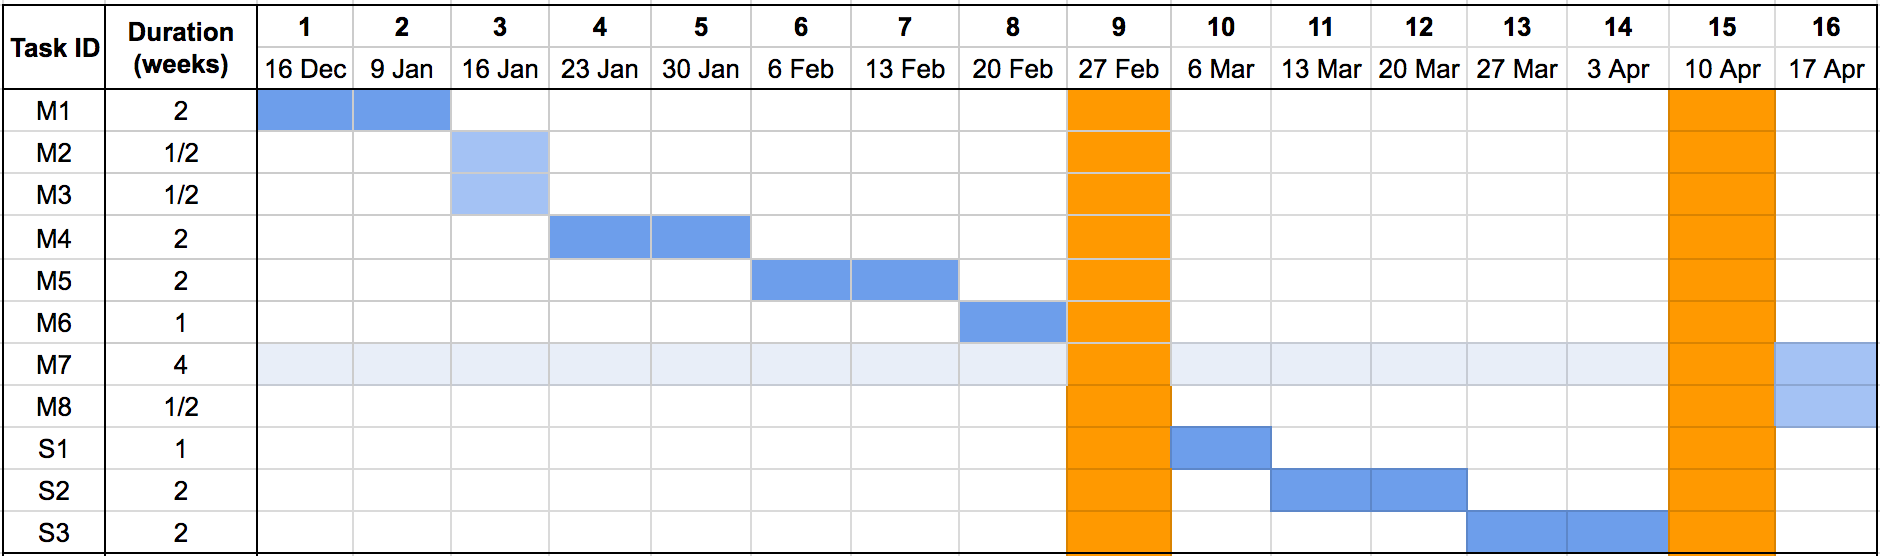
\includegraphics[width=16cm, height=6cm]{images/estimation.png}
\end{figure}

\clearpage

\newpage
%%%%%%%%%%%%%%%%%%%%%%%%%%%%%%%%%%%%%%%%%%%%%%%%%%%%%%%%%%%%%%%%%%%
% it is fine to change the bibliography style if you want
\bibliographystyle{plainnat}
\bibliography{mprop}
\end{document}
